\section{Droites particulières d'un triangle}

\dfnt{Hauteur}
{On appelle hauteur d'un côté d'un triangle la droite perpendiculaire à ce côté et passant par le sommet opposé.}
\rmq{Pour un triangle rectangle, deux des hauteurs sont des côtés du triangle.}


\dfnt{Médiane}
{On appelle médiane d'un côté d'un triangle la droite passant par le milieu de ce côté et passant par le sommet opposé.}

\prop{Aire d'un triangle}
    {\begin{multicols}{2}
        \begin{figure}[H]
            \centering
            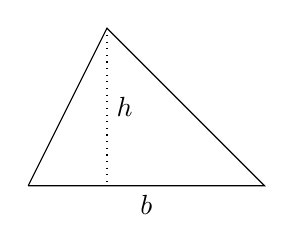
\begin{tikzpicture}
                \draw (0,0)--(1,2) --(3,0)--(0,0) node [midway, below] {$b$};
                \draw[dotted] (1,2)--(1,0) node [midway,right] {$h$};
                %\draw[dashed] (0,0) --(0,2)-- (3,2)--(3,0) ;
            \end{tikzpicture}
        \end{figure}
        \begin{figure}[H]
            \centering
            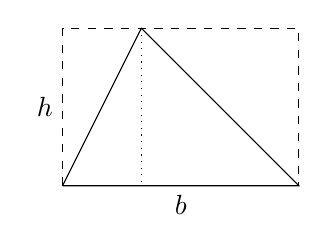
\begin{tikzpicture}
                \draw (0,0)--(1,2) --(3,0)--(0,0) node [midway, below] {$b$};
                \draw[dotted] (1,2)--(1,0);
                \draw[dashed] (0,0) --(0,2) node [midway,left ] {$h$} -- (3,2)--(3,0) ;
            \end{tikzpicture}
        \end{figure}
    \end{multicols}
    L'aire d'un triangle à l'aide de la formule $\text{Base}\times\text{Hauteur}\div 2=\dfrac{\text{Base}\times\text{Hauteur}}{2}$. Dans le cas de la figure ci dessus :
    $$\dfrac{b\times h}{2}$$
    }
\rmq{Aire d'un triangle rectangle}

